%
% wuerfel.tex
%
% (c) 2021 Prof Dr Andreas Müller, OST Ostschweizer Fachhochschule
%
\begin{frame}[t]
\frametitle{Würfelverdoppelung}
\vspace{-20pt}
\begin{columns}[t,onlytextwidth]
\begin{column}{0.48\textwidth}
\begin{center}
\begin{tikzpicture}[>=latex,thick]
\node at (0,0) {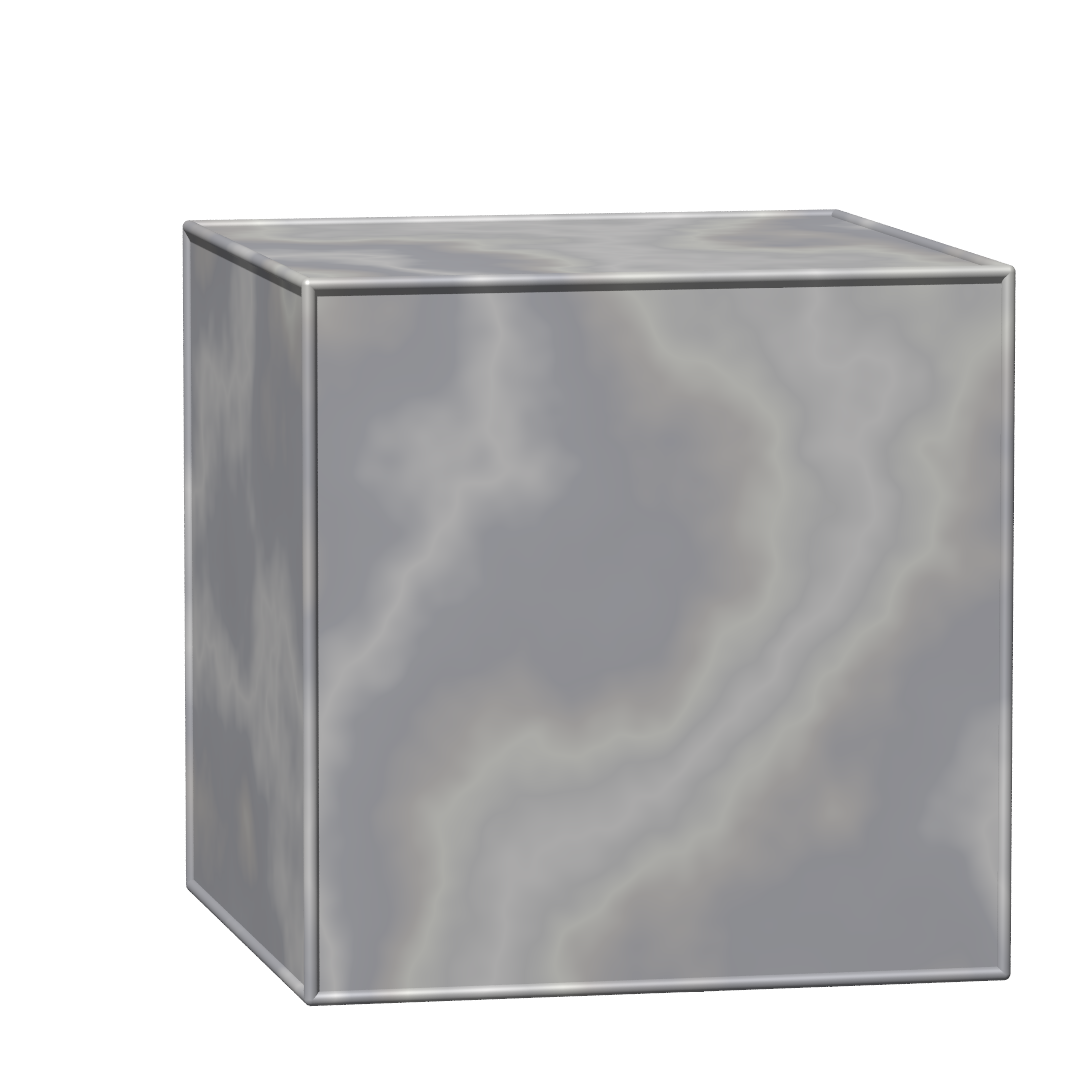
\includegraphics[width=6.0cm]{../slides/4/galois/images/wuerfel.png}};
\uncover<2->{
\node at (0,0) {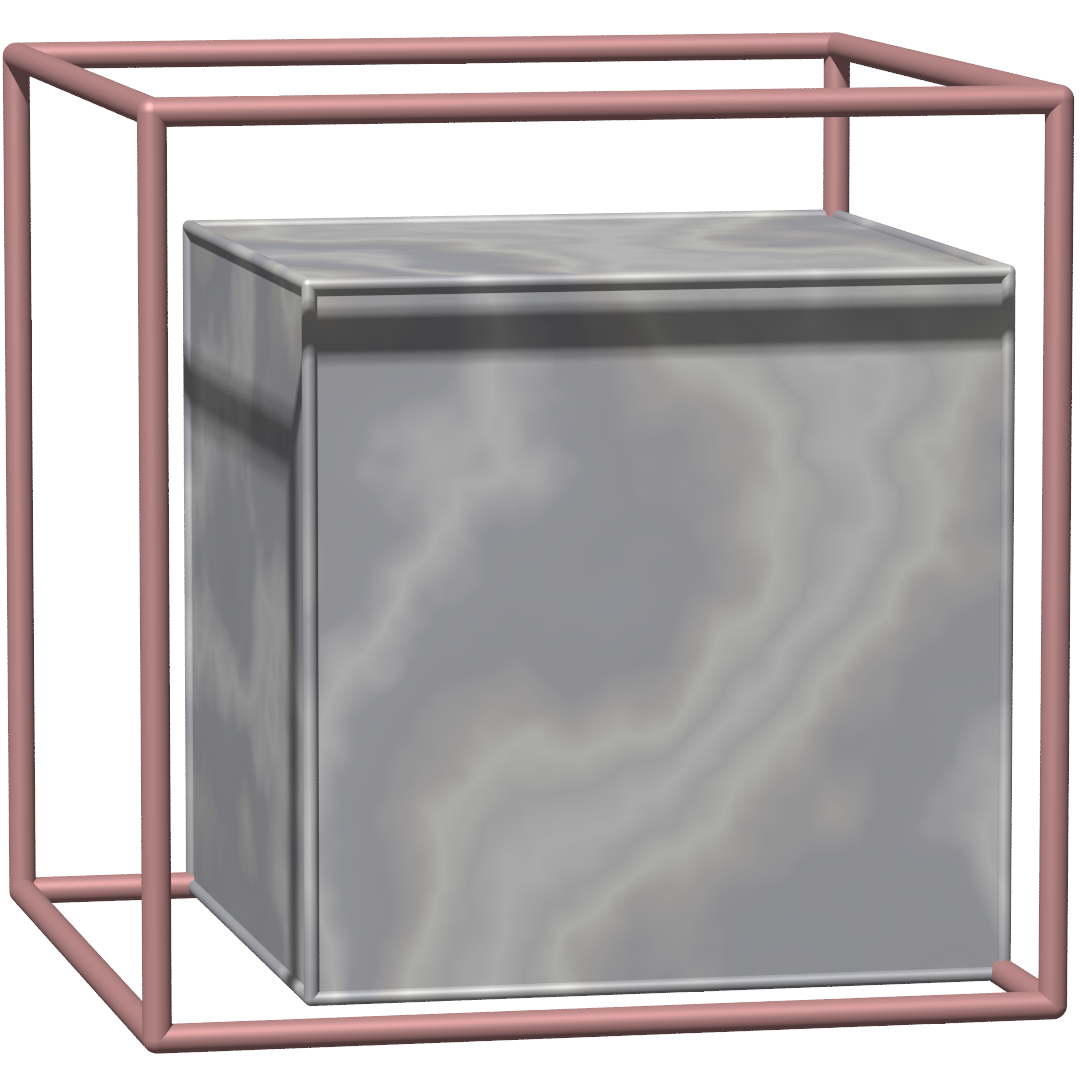
\includegraphics[width=6.0cm]{../slides/4/galois/images/wuerfel2.png}};
}

\uncover<3->{
	\draw[<->,color=blue] (-1.25,-2.4) -- (2.55,-2.25);
	\node[color=blue] at (0.75,-2.3) [above] {$a$};
}

\uncover<4->{
	\begin{scope}[yshift=0.03cm]
		\draw[color=red] (-2.13,-2.89) -- (-2.13,-3.19);
		\draw[color=red] (2.85,-2.7) -- (2.85,-3.0);
		\draw[<->,color=red] (-2.13,-3.09) -- (2.85,-2.9);
	\end{scope}
	\node[color=red] at (0.36,-2.9) [below] {$b$};
}

\uncover<5->{
\node at (0,-4) {$
	2{\color{blue}a}^3={\color{red}b}^3
	\uncover<6->{\;\Rightarrow\;
	\frac{b}{a} = \sqrt[3]{2}}$};
}

\end{tikzpicture}
\end{center}
\end{column}
\begin{column}{0.52\textwidth}
\begin{block}{Aufgabe}
Konstruiere einen Würfel mit doppeltem Volumen
\end{block}
\uncover<7->{%
\begin{block}{Algebraisierte Aufgabe}
Konstruiere eine Nullstelle von $p(x)=x^3-2$
\end{block}}
\uncover<8->{%
\begin{proof}[Unmöglichkeitsbeweis]
\begin{itemize}
\item<9->
$p(x)$ irreduzibel
\item<10->
$p(x)$ definiert eine Körpererweiterung vom Grad $3$
\item<11->
Nur Körpererweiterungen vom Grad $2^l$ sind konstruierbar
\qedhere
\end{itemize}
\end{proof}}
\end{column}
\end{columns}
\end{frame}
